\chapter{Resultados Obtidos}
\label{chap:resultados obtidos}

Neste capítulo, é apresentado as primeiras aplicações do catálogo, para isso então foi utilizado o conceito de personas \ref{sec:personas} buscando demonstrar os cenários em que o catálogo é aplicável. Portanto, realizou-se a simulação de cinco cenários para validar a aplicação do Catálogo de Segurança. 

O capítulo é divido inicialmente pelos cenários contextualizados dentro de cada persona. Em cada persona contém, a (i) descrição da persona, com problema, objetivo, desafio e possível solução, (ii) identificação da possível solução e (iii) aplicação do catálogo, finalizando e fechando o capítulo é apresentado a (iv) primeira visão da aplicação do catálogo.  


\section{Persona 1}

Heleno, 24 anos, Engenheiro de Requisitos está assumindo a função de elicitar os requisitos não funcionais para um novo projeto na empresa em que trabalha, o projeto será desenvolvido em \textit{Rails} e seu chefe pediu que devesse ter perfis diferentes dentro da aplicação sendo os perfis de membro e administrador. O sistema ao qual seu chefe está solicitando deve principalmente ser um sistema seguro para autenticar o usuário com capacidade de redefinir a senha do usuário, ser possível monitorar a quantidade de entradas do usuário e por final validar email do usuário.

\begin{itemize}
	\item O problema: Mapear os métodos de autenticação relevantes na autenticação do usuário. 
	\item Objetivo: Verificar o nível de satisfação de segurança da autenticação. 
	\item Desafio: Análise dos impactos entre os requisitos não funcionais para autenticar os usuários.
\end{itemize}


\subsubsection{Identificar possível solução}

O problema principal do usuário é a realização da autenticação do usuário o primeiro passo a ser adotado é identificar qual \textit{gem} é a mais adequada, segundo o \textit{The Ruby Toolbox} na categoria \textit{Rails Authentication} o ranking de popularidade das três \textit{gems} mais utilizadas para autenticação é \cite{rubytoolbox}:

\begin{enumerate}
	\item devise: 38.982.741 downloads
	\item omniauth: 23.524.509 downloads
	\item doorkeeper: 7.091.328 downloads
\end{enumerate}

Portanto, a \textit{gem} selecionada para ser aplicada ao projeto por Heleno é a \textit{devise}, pois além da posição do ranking é a \textit{gem} mais recomendada pela comunidade. As vantagens da utilização do \textit{devise} é  (i) uma solução baseada no padrão arquitetural MVC, (ii) permite a criação e a utilização de vários perfis de usuários conectados ao mesmo tempo, (iii) basea-se no conceito de modularidade, utilizando somente o que é necessário. Essa \textit{gem} possui 10 módulos \cite{gemdevise}: 

\begin{enumerate}
	\item \textit{Database Authenticatable}: \textit{Hashes} que armazenam a senha no banco de dados para serem validadas durante o \textit{login}. A autenticação pode ser realizada via método POST ou HTTP. 
	\item \textit{Omniauthable}: Suporte adicional ao \textit{omniauth}.
	\item \textit{Confirmable}: Envio automático de email para confirmação da conta e verificação da confirmação da conta durante o \textit{login}.
	\item \textit{Recoverable}: Envia instruções de redefinição de senha para o usuário e redefine a senha do usuário.
	\item \textit{Registerable}: Permite a inscrição de usuários por meio do processo de registros, permitindo a edição e a remoção de suas contas.
	\item \textit{Rememberable}: Gerenciador de \textit{token} para notificar o usuário da existência de \textit{cookie} salvo.
	\item \textit{Trackable}: contador de entradas, mantendo o registro de data, hora e endereço de IP.
	\item \textit{Timeoutable}: Expira as sessões inativas em um período de tempo especificado. 
	\item \textit{Validatable}: Validações de email e senha. 
	\item \textit{Lockable}: Bloqueia a conta após exceder o número de tentativas especificado, portanto o desbloqueio pode ocorrer via email ou após um período de tempo. 
\end{enumerate}

\subsubsection{Aplicação do Catálogo de Segurança}

Através dos módulos apresentados anteriormente é possível realizar o mapeamento deles utilizando o catálogo, então, modelou-se a \textit{gem devise} e seus respectivos métodos como operacionalizações no catálogo. 


\begin{figure}[h!]
	\centering
	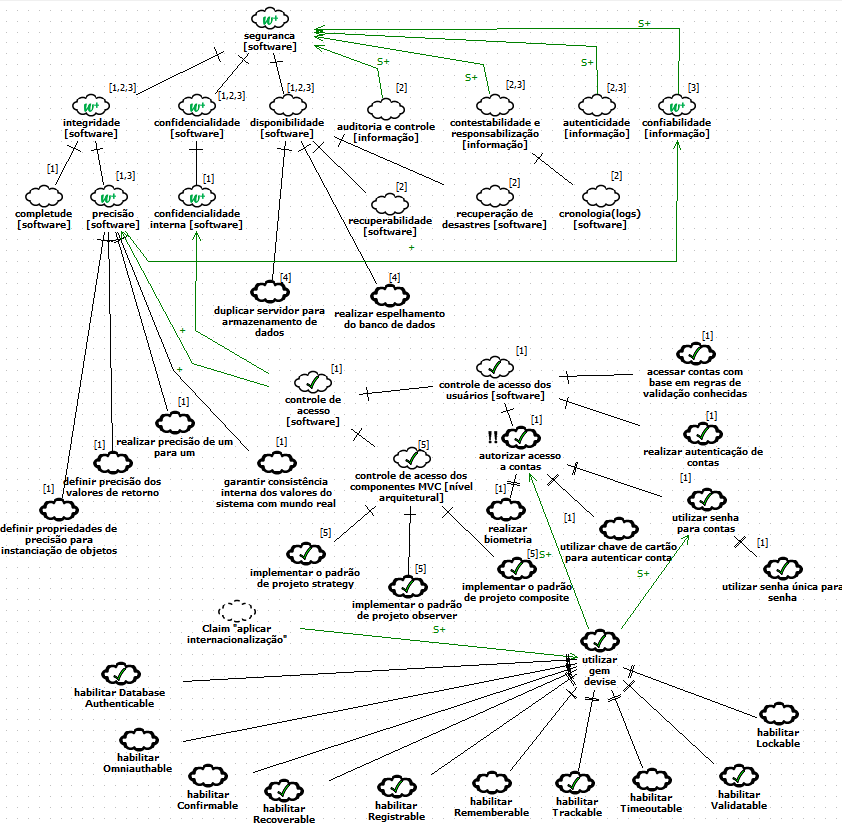
\includegraphics[keepaspectratio=true,scale=0.7]{figuras/catalogoPersona1.PNG}
	\caption{Operacionalizações para autenticação de usuário utilizando a \textit{gem devise}}
	\label{catalogoPersona1}
\end{figure}


O Catálogo de Segurança aplicado no cenário da \textit{Persona} 1 é apresentado na \ref{catalogoPersona1}, onde as operacionalizações são incrementadas no catálogo de respeitando os módulos do \textit{devise}, a operacionalização 'autorizar acesso a contas' passou a possui grau de prioridade alto, porquê é uma das operacionalizações que impactam diretamente a solução para o problema. 

É possível utilizando a notação do NFR \textit{Framework} realizar a modelagem da \textit{gem devise} como uma operacionalização, representando alguma contribuição positiva SOME+ com as operacionalizações 'autorizar acesso a contar' e 'utilizar senha para contas'.
 

As operacionalizações filhas de 'utilizar \textit{gem devise}' e que atendem as necessidades da \textit{Persona} 1 são:

\begin{itemize}
	\item habilitar \textit{Database Authenticable}: É um dos requisitos mínimos para que ocorra a persistência da senha no banco de dados.
	\item habilitar \textit{Recoverable}: Capacidade de redefinir a senha do usuário.
	\item habilitar \textit{Registrable}: É um dos requisitos mínimos e que permite a inscrição de usuários. 
	\item habilitar \textit{Trackable}: monitorar a quantidade de entradas do usuário. 
	\item habilitar \textit{Validatable}: Validar conta via email do usuário. 
\end{itemize}

Portanto ao habilitar os módulos do \textit{devise} dentro da \textit{model} nas classes Admins e Members, as operacionalizações são satisfeitas. Podemos então verificar o nível de segurança satisfeito com a utilização da \textit{gem devise}. O trecho de código abaixo apresenta como habilita-se os módulos.  
 

\begin{lstlisting} 
class Admins < ApplicationRecord
devise :database_authenticatable, :registerable,
:recoverable, :rememberable, :trackable, :validatable
end
\end{lstlisting} 

A implementação dos padrões de projeto \textit{strategy}, \textit{observer} e \textit{composite} já estão satisfeitos pois a aplicação é feita em MVC e a \textit{gem} que está sendo utilizada também percorre todas as camadas e é voltada para o padrão arquitetural MVC. 

\section{Persona 2}
\label{subsec:persona2}

Pedro, 23 anos, Engenheiro de Software, trabalha em empresa privada e possui a necessidade de desenvolver o sistema da ouvidoria da instituição, tal sistema deverá ser desenvolvido em plataforma web para atender os processos de manifestação (denúncia, reclamação, solicitação, sugestão e elogio) realizados pela ouvidoria. Esse tipo de informação deve ser estritamente confidencial, podendo ou não o manifestante ser anonimo.  

\subsection{Identificar possível solução}

Uma possível solução é gerar um número de protocolo durante o registro da manifestação para que possa ser realizado o acompanhamento, o manifestante poderá também acompanhar o status de sua manifestação através da visão de acompanhamento de manifestação, oinde ficará registrado respostas dada pela ouvidora.
A Ouvidora no caso acessará o sistema de maneira diferente, utilizando a área administrativa do sistema através de autenticação de usuário. 


\subsection{Aplicação do Catálogo de Segurança}

\begin{figure}[h!]
	\centering
	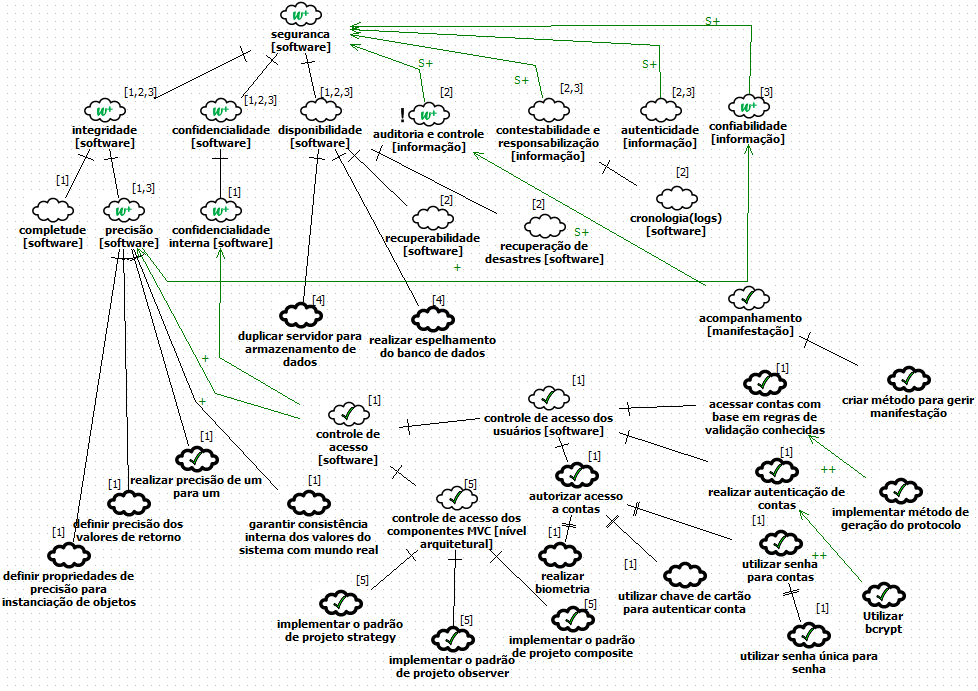
\includegraphics[keepaspectratio=true,scale=0.65]{figuras/catalogoPersona2.PNG}
	\caption{Catálogo de segurança aplicado ao sistema de ouvidoria.}
	\label{catalogoPersona2}
\end{figure}
\section{Persona 3}
\label{subsec:persona3}


Milena, 22 anos, Engenheira de Software, possui várias atividades no seu dia-a-dia, sentiu-se então a necessidade de organizar as suas atividades e para isso devido suas habilidades decidiu escrever um programa para obter maior controle. Esse programa descreve a atividade, a data de início, a previsão de conclusão e o status da atividade. Portanto, Gustavo optou por fazer seu sistema em Rails e decidiu verificar as relações entre as camadas do sistema com o foco em segurança.

\begin{itemize}
	\item O problema: Atividades diárias desorganizadas;
	\item Objetivo: Desenvolvimento de sistema para auxiliar na organização das atividades ;
	\item Desafio: Verificar as relações entre as camadas do sistema com foco em segurança
\end{itemize}

\subsubsection{Aplicação do Catálogo de Segurança}

Na descrição da persona tem se a necessidade de vincular cada atividade do mundo real com uma entidade no sistema, para isso utilizou se a ferramenta o Rails para 

\begin{figure}[h!]
	\centering
	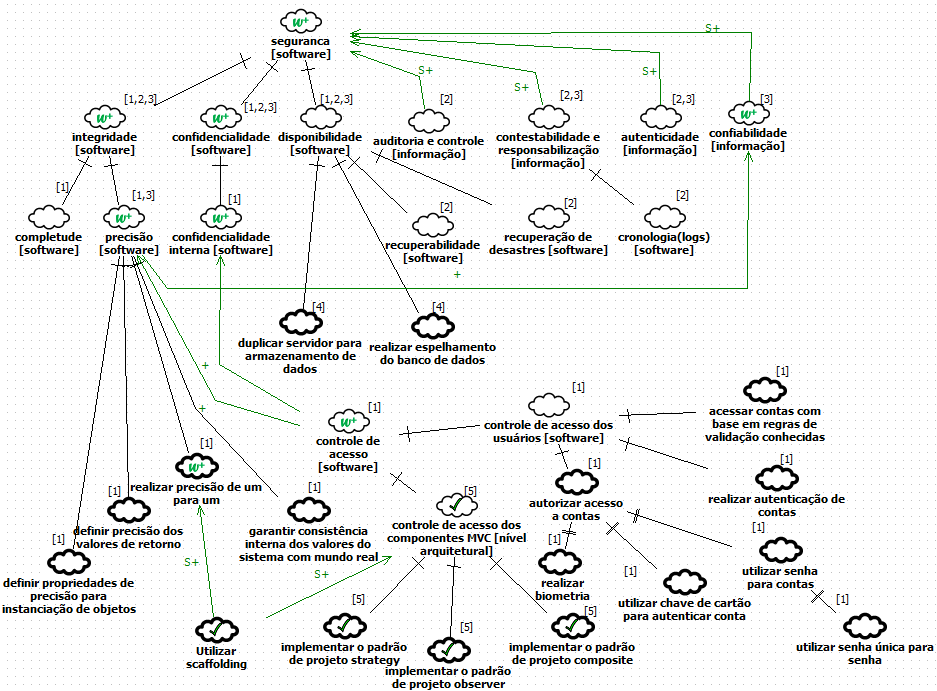
\includegraphics[keepaspectratio=true,scale=0.7]{figuras/catalogoPersona3.PNG}
	\caption{O scaffolding no catálogo.}
	\label{catalogoPersona3}
\end{figure}


\section{Persona 4}
\label{subsec:persona4}

<Escrever persona junto com o Vini>

Gustavo, 28 anos, Engenheiro de Requisitos, exerce a função em empresa privada onde foi demandado. 

\subsubsection{Identificar possível solução}

\subsubsection{Aplicação do Catálogo de Segurança}

\section{Persona 5}
\label{subsec:persona5}

Duplicação/espelhamento da base de dados. 

\subsubsection{Identificar possível solução}

\subsubsection{Aplicação do Catálogo de Segurança}


\section{Primeira visão da aplicação do catálogo}
\label{sec: aplicacaoDoCatalogo}
As atividades previstas para a execução do TCC1 de acordo com o cronograma apresentado na Tabela \ref{cronograma-tcc1} foram executadas com sucesso. Porém ao modelar a primeira versão do catálogo tem-se uma visão preliminar sobre Segurança devido a subjetividade e o conjunto de conceitos abstratos presentes na literatura.

A primeira versão do catálogo apresenta uma visão mais concreta para integridade de software e disponibilidade de software, onde o autor conseguiu detalhar em tempo de execução do TCC1 níveis de operacionalização com base na respectiva fonte ou referência teórica.

A Tabela \ref{resultadosObtidos} apresenta de acordo com os objetivos específicos do trabalho, usando "atendido", "parcialmente atendido" e "não atendido", os principais resultados obtidos até o momento, com a realização do TCC1.

\begin{table}[h!]
	\centering
	\caption{Resultados obtidos de acordo com os objetivos específicos.}
	\label{resultadosObtidos}
	\tiny
	\begin{tabular}{@{}p{6cm}p{3cm}p{6cm}@{}}
		\toprule
		\textbf{Objetivo} & \textbf{Nível de satisfação} & \textbf{Motivo} \\ \midrule
		Investigar na literatura formas de lidar com o RNF Segurança  em aplicações Web desenvolvidas utilizando o MVC. & Parcialmente atendido & Parcialmente atendido, pois existem fontes não confiáveis que comprovam o impacto do RNF Segurança com aplicações web desenvolvidas utilizando o MVC, um exemplo claro de fonte não confiável são os fóruns de dúvidas. Considera-se que ao desenvolver a aplicação fica mais evidente e possível comprovar as formas de lidar com o RNF segurança no Padrão arquitetural MVC. \\
		\rowcolor[HTML]{C0C0C0} 
		Investigar na literatura os RNF associados a segurança e identificar o impacto e as interdepêndencias entre eles. & Parcialmente atendido & Parcialmente atendido, pois a subjetividade dos RNFs para Segurança dificulta o tratamento, além de dificultar a identificação do impacto entre eles. \\
		Elaborar SIG & Atendido & Atendido, pois tem-se a primeira versão do catálogo elaborado com sucesso. \\
		\rowcolor[HTML]{C0C0C0} 
		Realizar correspondência entre o catálogo e as camadas do padrão arquitetural MVC & Atendido & Atendido, pois essa correspondência foi analisada de acordo com a base teórica já levantada. \\ \bottomrule
	\end{tabular}
\end{table}